%%%%%%%%%%%%%%%%%%%%%%%%%%%%%%%%%%%%%%%%%%%%%%%%%%%%%%%%
%%%%                                              %%%%%%
%%%%  Author: Peter Wilson                        %%%%%%
%%%%                                              %%%%%%
%%%%  Composite shells                        %%%%%%
%%%%                                              %%%%%%
%%%%%%%%%%%%%%%%%%%%%%%%%%%%%%%%%%%%%%%%%%%%%%%%%%%%%%%%


%fref generates automatically the respective abreviation/word in the text for the reference. You just have to define a label starting with the respective keyword.
%english: chap, sec, fig, eq, app
%deutsch: chap/kap, abs, abb, gl, anh
%see http://ctan.space-pro.be/tex-archive/macros/latex/contrib/fancyref/fancyref.pdf for more \section

%\onehalfspacing
%\setlength{\belowcaptionskip}{-17pt}

\chapter{Composite shells}
\label{chap:chapter_2_1}

\renewcommand{\Thema}{Composite shells}

\lettrine[lines=2]{A}{s} is the case with shell structures, composite materials are widely encountered throughout nature and man-made structures. Truly isotropic materials are relatively rare to find in naturally occurring structures, with the phenotypical material usually being anisotropic due to varying demands in different directions. Intuitively, inspecting nature suggests that the best material for a structure subject to spatially non-uniform requirements will be non-uniform itself. This same approach has recently began to dominate the cutting edge of man-made engineering structures where specialized high-performance is demanded, leading to greater adoption of composite materials. The increasing proportion of composite materials in the aerospace industry is but one example of their increasing traction.

\begin{figure}[H]
	\centering
	\def\svgwidth{\columnwidth}
	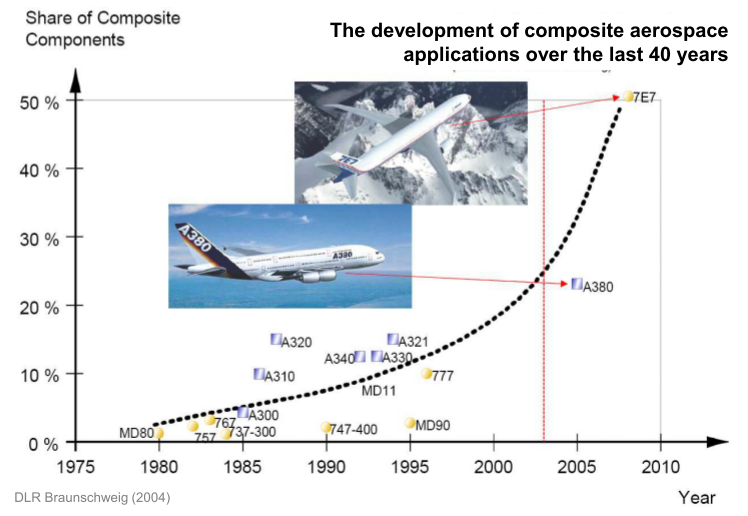
\includegraphics[width=12cm]{images/composites_aerospace.png}
	\caption{Proliferation of composite materials in the aerospace industry  \cite{BischLitBook04}}
	\label{composite_aerospace}
\end{figure}

The reason behind this increased propensity to use composites in high performance engineering applications is their customisability. Material properties such conductivity, density, wear resistance, and directional stiffness can be tailored to suit the exact needs of a design region. Directionally-varying stiffness is effectively leveraged in modern carbon-fiber road bicycles by simultaneously providing high stiffness for efficient power transfer and deliberate compliance for rider comfort and increased traction. This is one example of a composite material fulfilling seemingly mutually exclusive objectives due to finely tuned material properties built upon a knowledge of composite material basics.

\section{Composite material basics}

Composite materials are typically the combination of a high strength/stiffness fibre reinforcement material and a base matrix material which is usually weaker/softer than the fibres. Although a wide range composites exist, they are broadly grouped into fibrous composites (reinforcement material are fibres), particulate composites (reinforcement material are particles) and laminate composites composed of layers of different materials, including fibrous and particulate composites. Of these, this work focusses on laminates composed of fibrous composites which are commonly use in engineering.

\subsection{From laminae to laminates}

Laminae are individual layers or plies, which, when stacked together, form a laminate. Each lamina consists of a volume percentage of reinforcement fibres embedded within the matrix material aligned at a particular orientation to a common coordinate system. Common fibre reinforcement materials are various glass fibres (including E-glass and S-glass), carbon/graphite fibres and boron fibres while common matrix materials are thermosetting polymers such as polyester and epoxy resins and metals including aluminium and titanium. The reinforcement fibres may be arranged in the lamina matrix in a variety of patterns and orientations, either continuous or discontinuous \cite{agarwal2006analysis}. 
\begin{figure}[H]
	\subfloat[Composite laminae]
	{\label{ref_label2}
		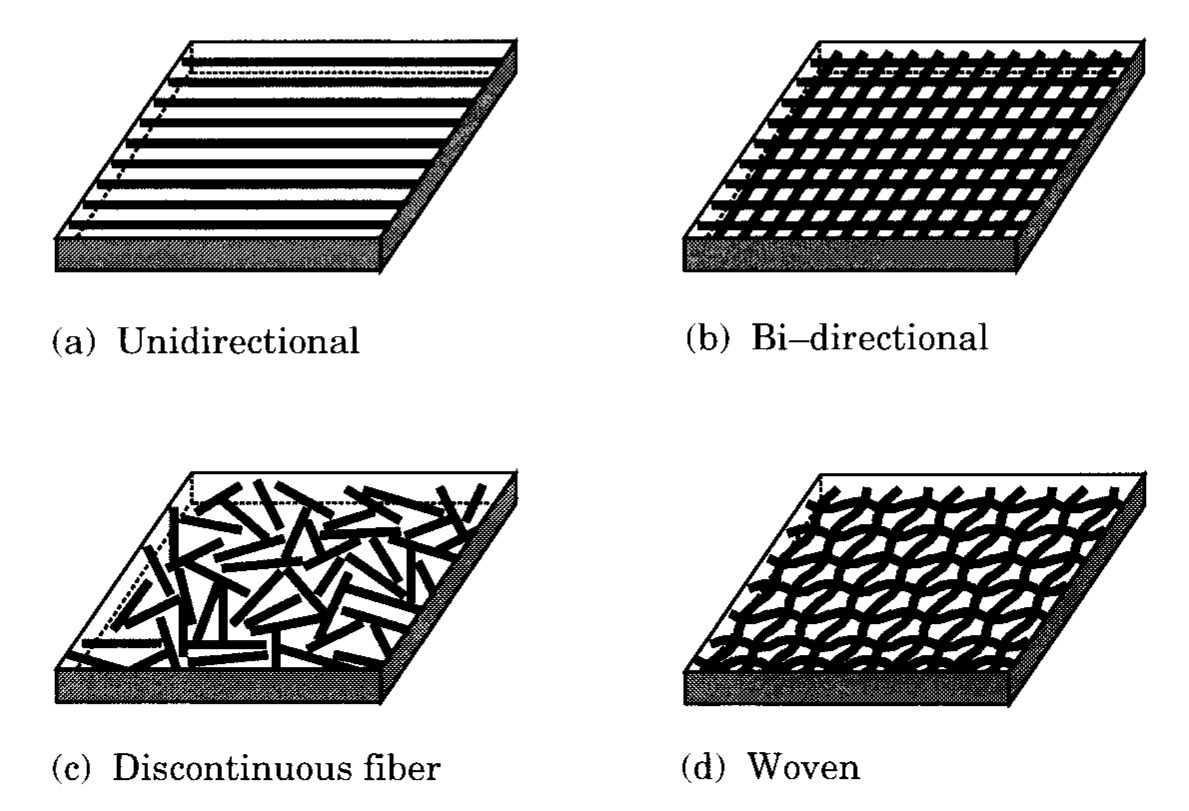
\includegraphics[width=7.3cm]
		{images/composite_laminae.png}}
	\subfloat[Composite laminate]
	{\label{ref_label2}
		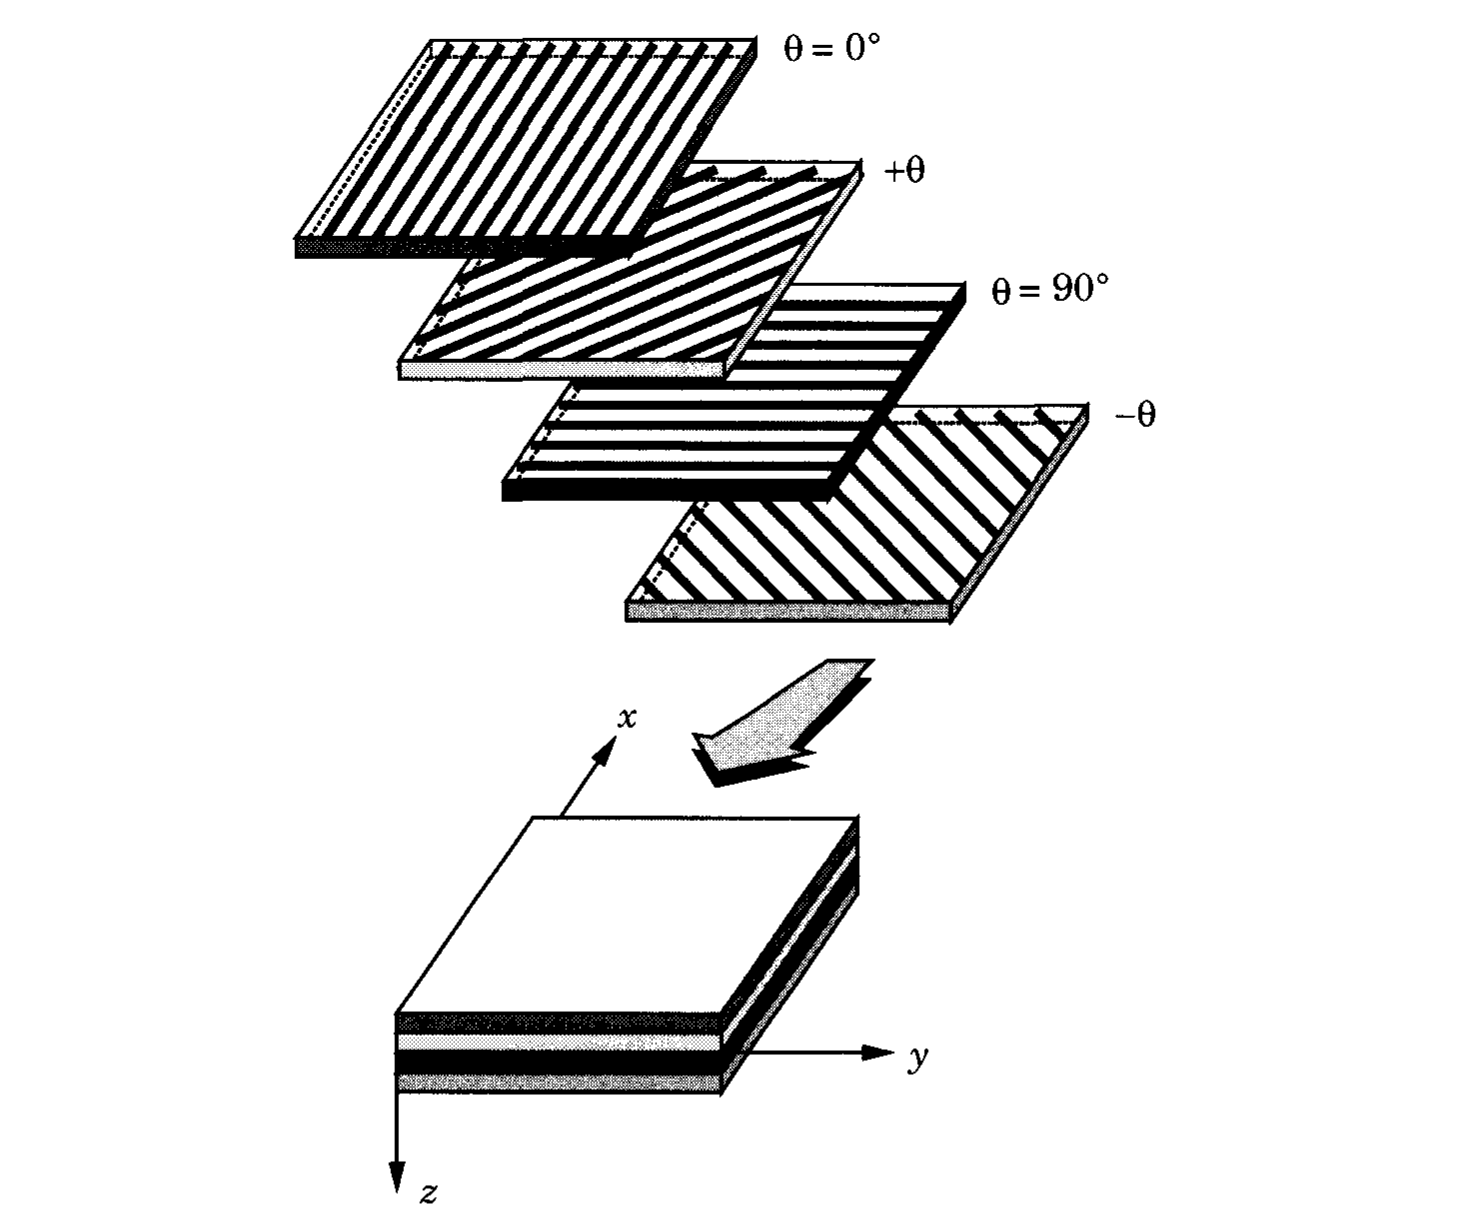
\includegraphics[width=7.3cm]
		{images/composite_laminates.png}}
	\caption{\label{composite_laminates}Components of composite laminates \cite{reddy2004mechanics}}
\end{figure}

Considering the four laminae in figure \ref{composite_laminates} examples of anisotropy to varying degrees can be intuited. The unidirectional continuous fibre pattern is incredibly stiff and strong in the fibre direction while being relatively compliant and weak  perpendicular to this fibre direction. Contrasting this, a practically in-plane isotropic lamina may be achieved with very fine discontinuous fibres randomly oriented within the matrix substrate. Thus, the importance of individual lamina makeup forms a critical determinant of the structural behaviour of the total laminate as a whole. Another critical determinant of the laminate behaviour is the stacking sequence of the laminate, which prescribes the number of laminae, their vertical order and their orientation. The control that these two determinants offer designers facilitate highly optimized structures for well defined structural requirements. An industrial example of this is spoolable Glass Reinforced Epoxy (GRE) oil piping which has a central structural lamina sandwiched between non-structural Polyethylene (PE) laminae intended to provide the structural layer chemical (inside) and environmental (outside) protection. Furthermore, the alignment of the GRE structural lamina is often orientated at an optimal pressure-capacity angle since the stress field of the pipe operating under internal pressure is well defined.

\subsection{Constitutive equations of a lamina}

 - Reddy ch 2.2 and ochoa reddy ch2.2 \cite{OchoaReddy92}
- Assumptions, General 3D law


- Generalized constitutive relations

\section{Orthotropic lamina}

- definition. plane stress, other assumptions or simplifications that come along with reducing complexity
-  constitutive relations Qij - stress and strain relations
	- transformation of strains
	- transformation of stresses

\section{Modelling of composite laminates}

- Integration of constitutive matrix


- Recovery of strains
\begin{figure}[H]
	\centering
	\def\svgwidth{\columnwidth}
	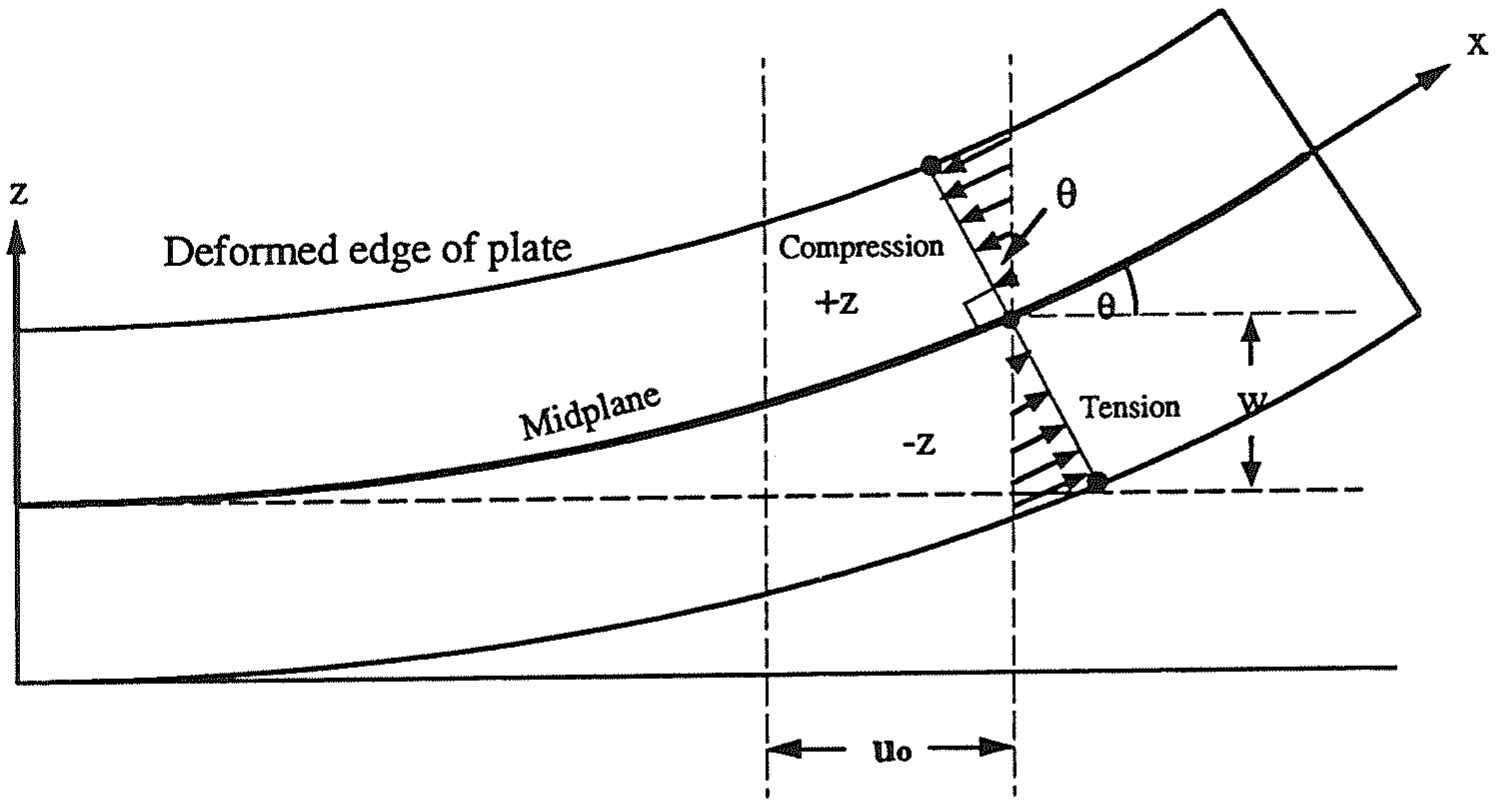
\includegraphics[width=12cm]{images/composite_nasa_strains.png}
	\caption{Deformation of 3 parameter plate \cite{nasanettles1994}}
	\label{fig:compositenasastrains}
\end{figure}

- Recovery of stresses 
\cite{agarwal2006analysis} eqn 6.9
\begin{figure}[H]
	\subfloat[Continuous strain distribution]
	{\label{ref_label2}
		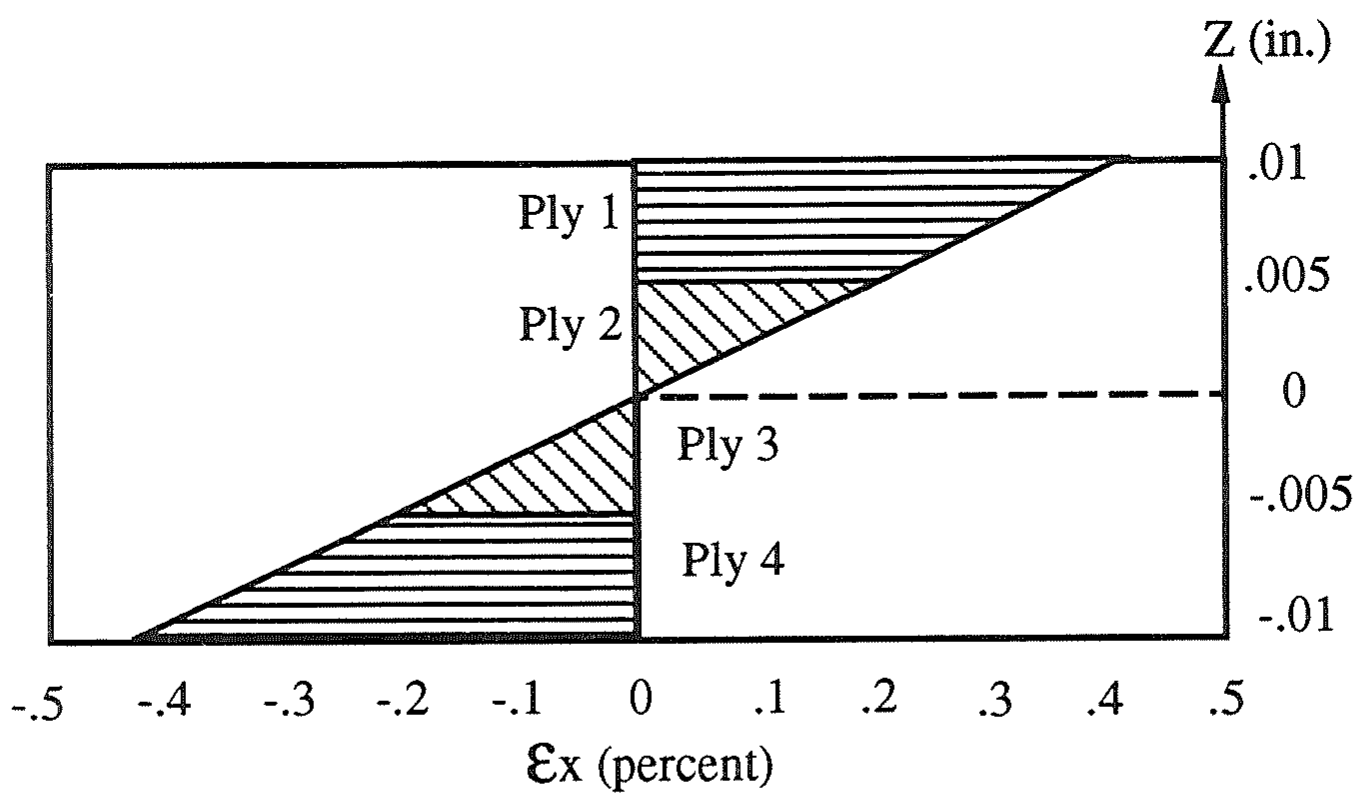
\includegraphics[width=7.3cm]
		{images/composite_nasa_strain_ex1.png}}
	\subfloat[Discontinuous stress distribution]
	{\label{ref_label2}
		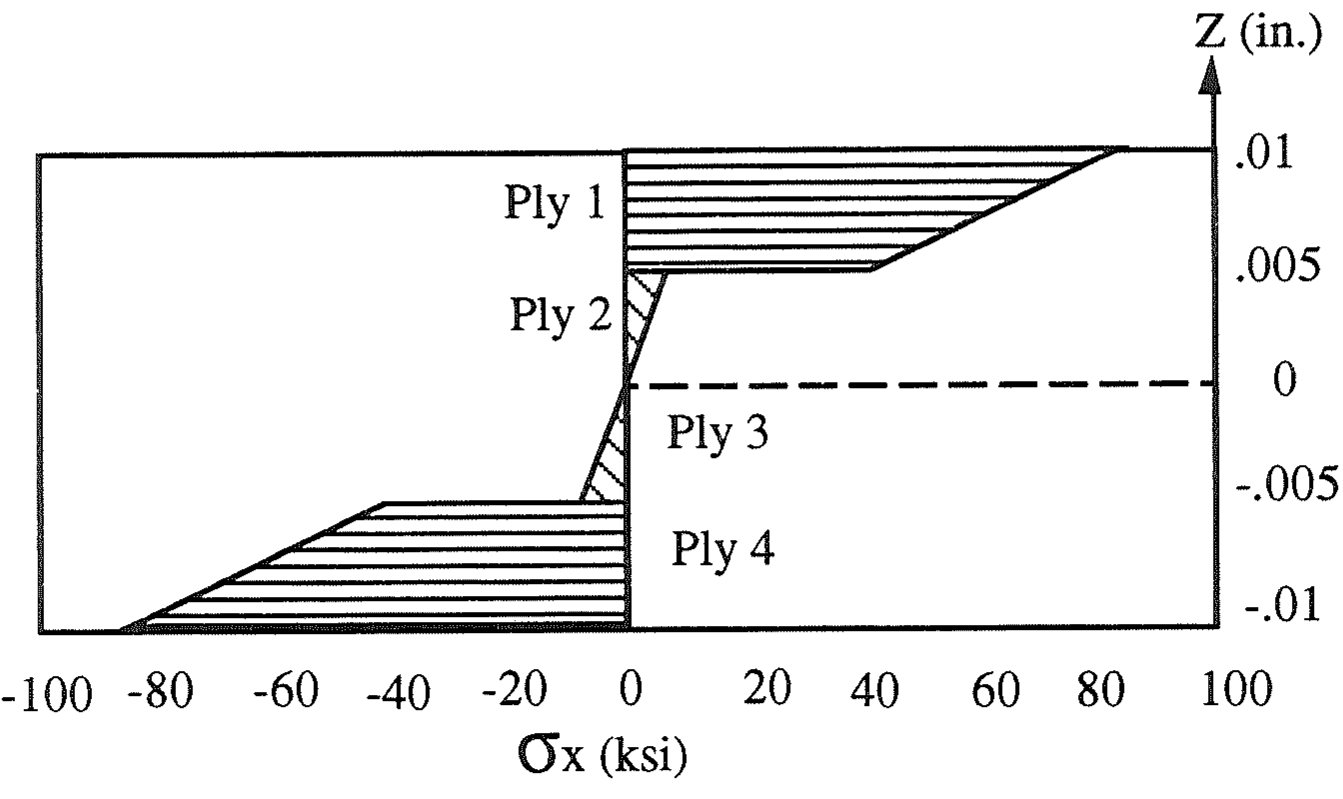
\includegraphics[width=7.3cm]
		{images/composite_nasa_stress_ex1.png}}
	\caption{\label{composite_stress_strain}Stress and strain thickness distribution of 4 ply plate subject to pure bending  \cite{nasanettles1994}}
\end{figure}
